%__begin__@TikzPy__#id__==__(0)
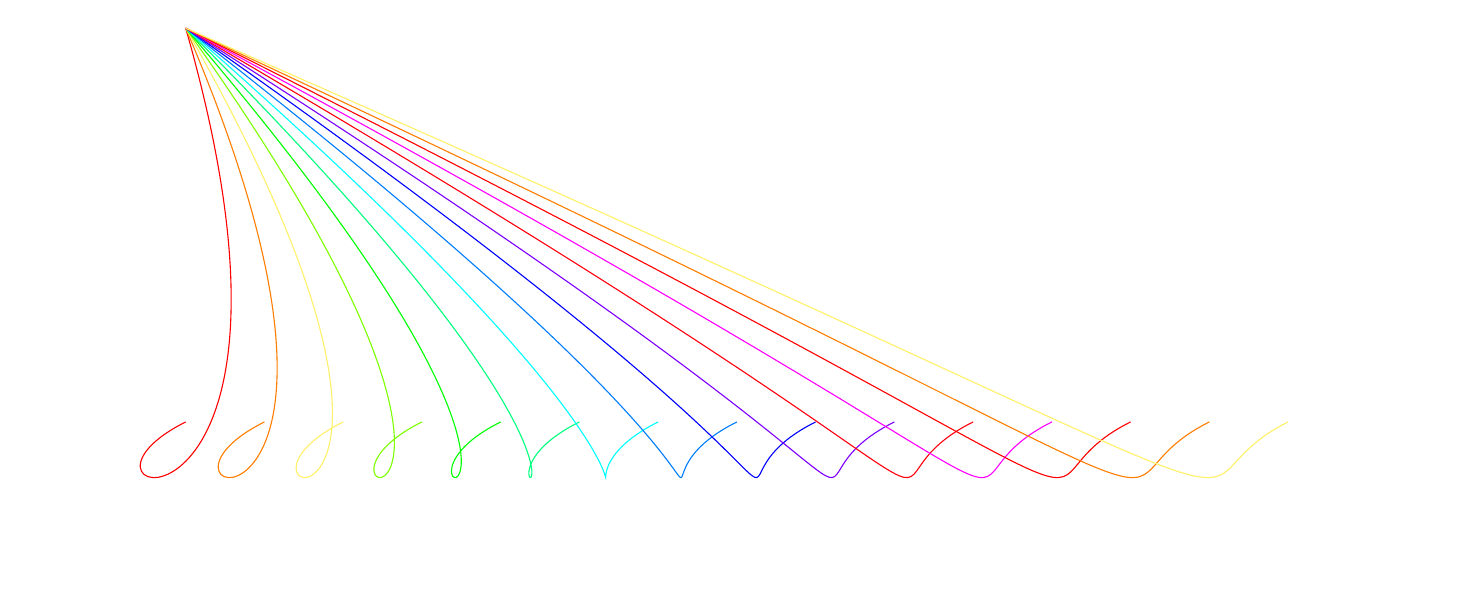
\begin{tikzpicture}
	\draw[color={rgb,255:red, 255; green, 0; blue, 0 }] (0, 0) .. controls (-2, -1) and (2, -2)  .. (0, 5);
	\draw[color={rgb,255:red, 255; green, 125; blue, 0 }] (1, 0) .. controls (-1, -1) and (3, -2)  .. (0, 5);
	\draw[color={rgb,255:red, 255; green, 240; blue, 105 }] (2, 0) .. controls (0, -1) and (4, -2)  .. (0, 5);
	\draw[color={rgb,255:red, 125; green, 255; blue, 0 }] (3, 0) .. controls (1, -1) and (5, -2)  .. (0, 5);
	\draw[color={rgb,255:red, 0; green, 255; blue, 0 }] (4, 0) .. controls (2, -1) and (6, -2)  .. (0, 5);
	\draw[color={rgb,255:red, 0; green, 255; blue, 125 }] (5, 0) .. controls (3, -1) and (7, -2)  .. (0, 5);
	\draw[color={rgb,255:red, 0; green, 255; blue, 255 }] (6, 0) .. controls (4, -1) and (8, -2)  .. (0, 5);
	\draw[color={rgb,255:red, 0; green, 125; blue, 255 }] (7, 0) .. controls (5, -1) and (9, -2)  .. (0, 5);
	\draw[color={rgb,255:red, 0; green, 0; blue, 255 }] (8, 0) .. controls (6, -1) and (10, -2)  .. (0, 5);
	\draw[color={rgb,255:red, 125; green, 0; blue, 255 }] (9, 0) .. controls (7, -1) and (11, -2)  .. (0, 5);
	\draw[color={rgb,255:red, 255; green, 0; blue, 12 }] (10, 0) .. controls (8, -1) and (12, -2)  .. (0, 5);
	\draw[color={rgb,255:red, 255; green, 0; blue, 255 }] (11, 0) .. controls (9, -1) and (13, -2)  .. (0, 5);
	\draw[color={rgb,255:red, 255; green, 0; blue, 0 }] (12, 0) .. controls (10, -1) and (14, -2)  .. (0, 5);
	\draw[color={rgb,255:red, 255; green, 125; blue, 0 }] (13, 0) .. controls (11, -1) and (15, -2)  .. (0, 5);
	\draw[color={rgb,255:red, 255; green, 240; blue, 105 }] (14, 0) .. controls (12, -1) and (16, -2)  .. (0, 5);
\end{tikzpicture}
%__end__@TikzPy__#id__==__(0)
